\documentclass[11pt]{article}
\usepackage[margin=1in]{geometry}
\usepackage[T1]{fontenc}
\usepackage{lmodern}
\usepackage{microtype}
\usepackage{amsmath}
\usepackage{booktabs}
\usepackage{graphicx}
\usepackage{xcolor}
\usepackage{xurl}
\usepackage[hidelinks]{hyperref}
\setlength{\emergencystretch}{2em}
\usepackage[numbers,sort&compress]{natbib}

\newcommand{\tps}{tok/s}

\title{Running, Pruning and Trying to Fine-Tune a 40B Mixture-of-Experts Model\\on a 24\,GB Mac with \$7 of Compute}
\author{Rinne (RINNECODER)\\\small\url{https://github.com/RINNECODER/flint-research}}
\date{October 2026}

\begin{document}
\maketitle

\begin{abstract}
We report a week of work on Flint, a 40B-parameter mixture-of-experts (MoE) language model with about 2.5B active
parameters per token, on a single 24\,GB Apple-silicon laptop and roughly \$6.8 of rented GPU time. We had three goals:
run the model fast enough to use, make it smaller without losing coding quality, and tune it into a stronger coding
agent. For speed, streaming routed experts from SSD, packing each expert into one contiguous read, a 6\,GB GPU expert
cache and DFlash~2 block-diffusion speculative drafts (width 2) took decode from about 10 to 32--36\,\tps{}, and pruning
32 of 256 experts per layer with REAP took it to 36.8\,\tps{}. The pruned model (REAP-224) lost one of 40 HumanEval+
tasks (36$\to$35), within noise, and stayed closer to the original model (KL 0.92 nats/token, 78.0\% top-1 agreement)
than frequency, random, or a published third-party mask. That third-party mask did no better than random on our
coding text. Both fine-tuning attempts made the model worse. Expert-specialized fine-tuning (ESFT) on verified
DeepSeek-R1 traces cut validation NLL from 0.956 to 0.529 but moved paired HE+/MBPP+ plus-test accuracy from 83.3\% to
81.3\% ($n{=}96$, $p{=}0.75$) and made replies 55\% longer. LoRA SFT on public frontier-model agent traces cut validation NLL
from 1.462 to 1.062 and dropped accuracy to 72.9\% ($p{=}0.013$) with replies 46\% shorter. We read these as findings
about off-policy imitation of a strong base, not as evidence that the model cannot be tuned. The work stopped when the
compute budget ran out; an on-policy DPO run was fully prepared and never executed.
\end{abstract}

\section{Introduction}

Open MoE models now approach frontier quality at a fraction of the active parameters, which makes them interesting for
consumer hardware: a model that computes like a 2.5B dense model can, in principle, decode at interactive speed if its
weights can be fed to the GPU fast enough. The catch is memory. Flint~\citep{flint} in its 4-bit release takes about
21\,GB, which does not fit next to an operating system in 24\,GB of unified memory.

This report covers three questions we tried to answer on that hardware, with almost no money:

\begin{enumerate}
  \item \textbf{Can a 40B MoE run usefully on a 24\,GB Mac?} Yes: by streaming routed experts from SSD, with a GPU
        expert cache and speculative drafts, it decodes at 32--36\,\tps{} (Section~\ref{sec:system}).
  \item \textbf{Can it be made smaller for coding work without measurable loss?} Removing 12.5\% of routed experts with
        REAP~\citep{lasby2025reap} cost one HumanEval+ task of 40 and gave a 14\% speedup (Section~\ref{sec:prune}).
  \item \textbf{Can it be tuned into a better coding agent?} We wanted a ``Qwythos-style'' tune: a community coding-agent
        fine-tune that imitates frontier-model agent traces. Two cheap attempts (ESFT and LoRA SFT) both made it worse
        (Section~\ref{sec:ft}). The budget ran out before the on-policy follow-up.
\end{enumerate}

We present the negative results with the same care as the positive ones. All numbers come from logs in the repository;
where a number rests on notes rather than a log we say so. Sample sizes are small and the fine-tuning runs are single
runs, so we give $n$, confidence intervals and paired tests throughout.

\section{Background}

\paragraph{Flint.} Flint is a Qwen3-MoE-style~\citep{qwen3} decoder with 49 layers: two dense SwiGLU layers and 47 MoE
layers, each with 256 routed experts (intermediate size 512), sigmoid routing with the top 6 renormalized, and one
ungated shared expert (intermediate size 1024). Attention has 32 query and 4 KV heads with a learned per-head sink logit;
35 layers use a 513-token sliding window with RoPE and 14 use full attention without RoPE. The vocabulary has 150,144
tokens. About 2.5B of the 40B parameters are active per token. We used the int4 release layout (MLX affine 4-bit, group
size 64, 8-bit embedding), mostly through an abliterated build with the same layout~\citep{abliterated}.

\paragraph{Expert streaming.} Because each token touches only 6 of 256 experts per layer, the routed experts can live on
SSD and be read on demand, while attention, router, shared experts and embeddings stay resident. This is the
flash-offloading idea of \citet{alizadeh2023flash} applied to MoE experts. We used Locals~\citep{locals}, an
Apache-2.0 MLX server that implements it.

\paragraph{Speculative decoding.} A cheap drafter proposes tokens and the full model verifies them in one pass; at
temperature 0 the output is unchanged~\citep{leviathan2022spec,chen2023specsampling}. DFlash~\citep{chen2026dflash}
drafts a block of tokens in one pass of a small block-diffusion model conditioned on the target's hidden states. A Flint
drafter (5 layers, 0.4B, bf16) is public~\citep{flintdflash2}.

\paragraph{REAP.} Router-weighted Expert Activation Pruning~\citep{lasby2025reap} scores each expert by the mean, over the
tokens routed to it, of its gate weight times the norm of its output, and removes the lowest-scoring experts
one-shot, with no retraining.

\paragraph{ESFT.} Expert-Specialized Fine-Tuning~\citep{wang2024esft} trains only the routed experts that carry most of the
gate mass on the task data and freezes the rest, which limits forgetting and memory.

\section{System: streaming plus drafting on Apple silicon}
\label{sec:system}

The machine was an M5 Pro laptop with 24\,GB of unified memory. We left the GPU wired-memory limit at its default.

\paragraph{The speed path.} Table~\ref{tab:speed} and Figure~\ref{fig:speed} show each step.
\begin{itemize}
  \item \emph{Stock streaming} from the safetensors shards gave about 10\,\tps{}. Each expert is nine slices spread over
        nine tensors, so one expert costs four or more reads.
  \item \emph{Expert pack} (\texttt{python -m locals.models.pack}) writes one file per layer laid out expert by expert,
        so an expert is one contiguous read: about 22\,\tps{}.
  \item \emph{GPU expert cache:} a 6\,GB LRU cache of experts in GPU memory plus a 2\,GB prompt cache (about 7.8\,GB
        resident) gave about 28\,\tps{}. An 8\,GB cache gave 31--32\,\tps{}; we kept 6\,GB to keep memory pressure low.
  \item \emph{DFlash~2 drafts.} We ported the DFlash MLX drafter into Locals (patches in the repository). The drafter
        reads Flint's hidden states at layers 5, 15, 26, 36 and 46. With streamed experts, a verify pass costs about
        60\,ms plus about 20\,ms per drafted token (each extra token pulls in more experts), against about 7\,ms for the
        drafter, so drafting 2 tokens per pass beat the default 7. Acceptance was 0.64. Two measurement sessions gave
        30.1 and 34.5\,\tps{} (mean 32.3).
  \item \emph{REAP-224} (Section~\ref{sec:prune}) gave 36.8\,\tps{} in both of two sessions, with acceptance 0.68.
\end{itemize}

The first three steps rest on notes taken during development, not on saved logs, and were measured on different days.
Only the last two rows have logs (\texttt{results/prune/*/speed\_\{on,off\}.log}): \texttt{prune/speed.py}, 2 coding
prompts $\times$ 2 runs, temperature 0, 1,024 new tokens, decode time from first to last streamed token. SSD and thermal
state move these numbers by about $\pm$10\%. On agent file rewrites, where the output copies the input, prompt-lookup
drafts reached about 46\,\tps{} (notes only).

\begin{table}[t]
\centering
\caption{Decode speed on a 24\,GB M5 Pro, experts streamed from SSD. Rows marked ``notes'' have no saved log.}
\label{tab:speed}
\begin{tabular}{lrrl}
\toprule
step & \tps{} & draft accept. & source \\
\midrule
stock streaming & $\sim$10 & -- & notes \\
+ expert pack & $\sim$22 & -- & notes \\
+ 6\,GB GPU expert cache & $\sim$28 & -- & notes \\
256 experts, no drafts (2 sessions) & 25.4 / 29.3 & -- & log \\
+ DFlash~2, width 2 (2 sessions) & 30.1 / 34.5 & 0.64 & log \\
REAP-224, no drafts (2 sessions) & 30.1 / 30.4 & -- & log \\
REAP-224 + DFlash~2 (2 sessions) & \textbf{36.8} / \textbf{36.8} & 0.68 & log \\
\bottomrule
\end{tabular}
\end{table}

\begin{figure}[t]
\centering
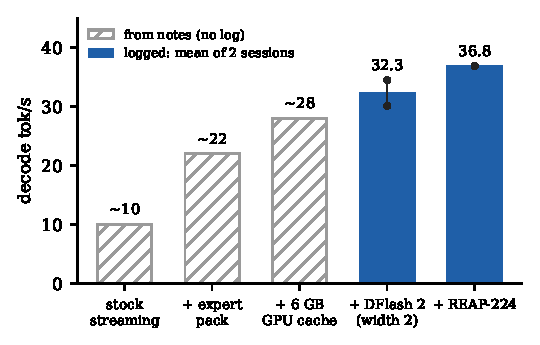
\includegraphics[width=0.6\linewidth]{figs/speed_path.pdf}
\caption{The speed path. Hatched bars come from development notes; solid bars are the mean of two logged sessions,
with the four individual runs as dots.}
\label{fig:speed}
\end{figure}

\paragraph{Correctness fixes.} Two bugs surfaced on the way. A rejected draft left stale keys in Flint's sliding-window
ring buffers because the cache was trimmed from the ring length rather than its index; and a prompt-cache entry reused as
a strided KV view raised a contiguity error that surfaced as an HTTP 500. Both are fixed in the published patches.

\paragraph{Things that did not help.} A RAM tier for experts was slower; page-cache reads instead of uncached reads were
neutral; Locals' other scheduling knobs were best at their defaults.

\section{Expert pruning}
\label{sec:prune}

Fewer distinct experts per layer means less to stream and more cache hits. We pruned on the Mac, in-process on the
streamed model, with no GPU rental.

\subsection{Method}

\paragraph{Data.} Calibration used 217,606 tokens of coding and coding-agent text: Python source (codeparrot), SWE-agent
trajectories (nebius) and OpenHands trajectories (SWE-Gym), about 70k tokens each, rendered with the model's chat
template. Evaluation used 32 disjoint held-out windows of 1,025 tokens (11/11/10 per source).

\paragraph{Statistics and masks.} For each MoE layer and expert we recorded routing count, summed gate weight, and summed
gate $\times$ output norm. We compared, at 224 experts per layer: REAP (mean of gate $\times$ norm over routed tokens),
sum-REAP (the same sum, which weights by frequency), routing frequency, random, and the published RESMP RCO-224
mask~\citep{resmp}, which was built for the original (not abliterated) Flint with a different objective and data. We then
pruned REAP iteratively, 224$\to$192$\to$160, re-scoring on the parent each time. Pruning slices the expert tensors and
router rows as raw bytes, so the result keeps the int4 layout.

\paragraph{Metrics.} The reference is the 256-expert model, not the text, so we report per-token KL(256\,$\|$\,variant)
and top-1 agreement on the held-out windows, with a window-level bootstrap CI. The noise floor is not zero: re-running
the 256-expert model with chunked prefill alone gives KL 0.42 and 85.8\% agreement. HumanEval+~\citep{liu2023evalplus,chen2021humaneval}
used every fourth task (40), greedy with full reasoning and drafts on, through the Locals server.

\subsection{Results}

\begin{table}[t]
\centering
\caption{Pruning results on held-out coding and agent text. KL in nats/token with 95\% bootstrap CI over 32 windows.
HE+ is plus-test pass@1 on 40 tasks with Wilson 95\% CI. ``Dropped slots'' is the share of calibration routing slots
that went to removed experts, computed from \texttt{prune/stats/stats\_256experts.npz}.}
\label{tab:prune}
\resizebox{\linewidth}{!}{%
\begin{tabular}{lrrrrr}
\toprule
variant & KL (95\% CI) & top-1 agree & dropped slots & HE+ plus (n=40) & \tps{} drafts on / off \\
\midrule
256, chunked prefill (noise floor) & 0.42 [0.31, 0.54] & 85.8\% & 0 & -- & -- \\
256 (original) & -- & -- & 0 & 36 [77\%, 96\%] & 32.3 / 27.3 \\
\textbf{REAP-224} & \textbf{0.92} [0.71, 1.14] & \textbf{78.0\%} & 10.1\% & 35 [74\%, 95\%] & \textbf{36.8} / 30.3 \\
sum-REAP-224 & 0.90 [0.70, 1.12] & 78.0\% & 4.5\% & -- & -- \\
frequency-224 & 0.98 [0.79, 1.18] & 75.4\% & 3.5\% & -- & -- \\
RESMP RCO-224 & 1.49 [1.25, 1.75] & 68.3\% & 12.3\% & -- & -- \\
random-224 & 1.47 [1.21, 1.73] & 68.6\% & 12.6\% & -- & -- \\
REAP-192 & 1.21 [0.96, 1.47] & 73.7\% & 19.3\% & 32 [65\%, 90\%] & 36.5 / 31.6 \\
REAP-160 & 1.45 [1.18, 1.74] & 69.9\% & 28.4\% & 29 [57\%, 84\%] & 38.3 / 33.1 \\
\bottomrule
\end{tabular}}
\end{table}

\begin{figure}[t]
\centering
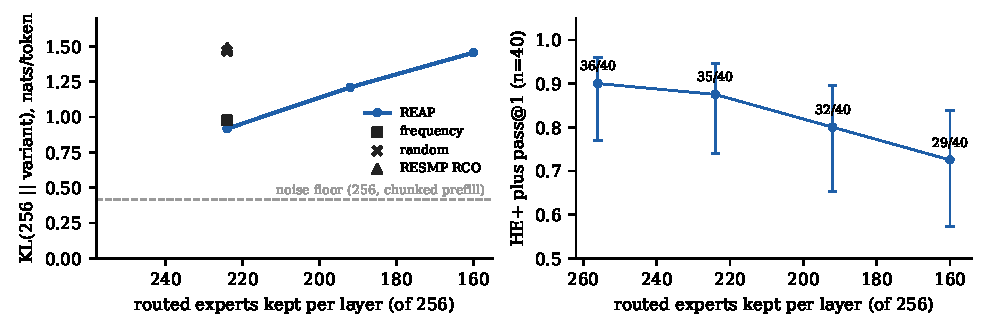
\includegraphics[width=\linewidth]{figs/pruning.pdf}
\caption{Left: divergence from the 256-expert model as experts are removed, with the three alternative masks at 224.
Right: HumanEval+ plus pass@1 on 40 tasks with Wilson 95\% intervals.}
\label{fig:prune}
\end{figure}

Table~\ref{tab:prune} and Figure~\ref{fig:prune} give the results.

\begin{itemize}
  \item \textbf{REAP and sum-REAP tie at 224 and beat frequency}, though frequency is only modestly worse. All three are
        about twice the noise floor in KL.
  \item \textbf{REAP-224 lost one HumanEval+ task} (36$\to$35 of 40; the base-test count stayed at 37). With $n{=}40$ the
        intervals overlap almost completely, so we claim only that no large regression is visible.
  \item \textbf{REAP-224 is 14\% faster} with drafts (32.3$\to$36.8\,\tps{}), 12\% smaller on disk (about 19 vs 21\,GB),
        and has higher draft acceptance (0.68 vs 0.64). The speedup is consistent with fewer distinct experts giving more
        cache hits; we did not measure hit rates.
  \item \textbf{Going further buys little speed.} REAP-192 is no faster than REAP-224 with drafts, because acceptance
        falls to 0.61. REAP-160 gains 4\% speed for 6 lost tasks against the original. Acceptance is 0.61 at both 192
        and 160.
  \item \textbf{REAP does not simply drop rare experts.} The experts REAP-224 removes still carried 10.1\% of routing slots,
        against 3.5\% for frequency pruning. REAP keeps some rarely routed experts whose outputs matter when they fire, and
        it is still closer to the original model.
\end{itemize}

\paragraph{Negative result: the RESMP mask.} The published RCO-224 mask scored KL 1.49 and 68.3\% agreement, the same as a
random mask (1.47, 68.6\%). Its removed experts carried 12.3\% of routing slots on our calibration text, which is what a
random 224-of-256 mask removes in expectation (12.5\%; our random draw: 12.6\%). On this model and this text it carries no
information about which experts matter. This is not evidence against that method on its own target: the mask was
optimized for the original Flint's GPTQ-MXFP4 build, with a different objective and data.

\paragraph{NLL against text is misleading here.} Random and RESMP masks have \emph{lower} NLL on the held-out text
(2.93 and 3.06 vs 3.28 for 256 experts) while diverging most from the base model. Matching the model, not the text, is the right target for a lossless-ish compression.

REAP-224 is published on Hugging Face (Section~\ref{sec:repro}).

\section{Fine-tuning attempts}
\label{sec:ft}

\subsection{An int4 PyTorch reimplementation}

To train without dequantizing the whole model to bf16 (about 80\,GB), we wrote Flint from scratch in PyTorch so that it runs directly on the packed weights:
\begin{itemize}
  \item weights stay packed and are dequantized inside the forward pass, so the 40B model fits on one 48\,GB A6000 with
        room for training, or on two 16\,GB T4s;
  \item attention uses SDPA's memory-efficient kernel with the sink as an extra key, so 6k-token sequences fit;
  \item LoRA~\citep{hu2021lora} can sit on attention and the shared expert, and selected routed experts can be unpacked
        to bf16 and trained;
  \item trained weights are re-quantized into the checkpoint's own keys and patched in byte for byte, so the result
        loads in Locals unchanged.
\end{itemize}
Parity: on a tiny random Flint built with Locals' MLX model, logits match within 0.3\% relative error with 100\% top-1
agreement. On the full model, a free Kaggle 2$\times$T4 kernel reproduced Locals' greedy continuations with 96.9\%
top-1 agreement over 32 tokens on 3 prompts. A JAX port for a Kaggle TPU v5e-8 never got a TPU slot: the probe waited
about 20\,h in the queue and the proof kernel more than 24\,h, so the JAX path is tested only on CPU.

The T4s were too slow for real runs (39\,s per 2k-token LoRA step, about 54 GPU-hours per 5k examples), so training moved
to rented RTX A6000s on Lium at \$0.42/h.

\subsection{Evaluation protocol}

All training evals use one fixed seed-0 sample of 48 HumanEval+ and 48 MBPP+~\citep{austin2021mbpp,liu2023evalplus}
problems ($n{=}96$), greedy decoding with thinking on and a 4,096-token cap. We score the longest Python block after the
thinking section against both the original (``base'') tests and the stricter ``plus'' tests. Each tuned model is
compared, item by item, with the same base model: we report the paired difference with a bootstrap 95\% CI,
wins/losses, and an exact McNemar $p$-value. The base model scores 83.3\% plus and 92.7\% base, with a mean reply of
972 tokens.

\subsection{ESFT on verified R1 traces}

We summed routed gate mass per expert over the training data (301,827 tokens) and kept, per layer, the experts holding
the top 20\% of gate mass: 593 experts, 1.87B parameters. Data: 2,144 DeepSeek-R1~\citep{deepseekr1} competitive-programming
traces (4.4M tokens) from public sets, each verified by running its code on tests, 27\% wrapped as synthetic tool-use
trajectories, and 13-gram decontaminated against HE+/MBPP+. Training: one epoch (268 steps), LR $10^{-5}$ cosine, batch
8 by accumulation, bf16 Adam moments with stochastic rounding, 4\,h\,55\,min on one A6000.

\subsection{LoRA SFT on frontier-model traces}

LoRA with rank 32 and $\alpha{=}64$ on q/k/v/o and the shared expert (42.7M parameters); routed experts frozen int4.
Data: 2,053 examples (5.8M tokens, 6,144-token cap): about 1,020 public agentic tool-use trajectories attributed to a
frontier Claude model, mapped onto one bash, read, write, edit, grep and glob toolset, and 1,033 public coding-chat answers
attributed to Claude Opus models. Training: 218 steps on 85\% of the data, LR $10^{-4}$ cosine, 307\,min on one A6000.

\subsection{Results}

\begin{table}[t]
\centering
\caption{Fine-tuning results, $n{=}96$ HE+/MBPP+ items paired against the same base model. CIs are bootstrap 95\%;
$p$ is exact McNemar. Val NLL is on held-out teacher traces (bf16 weights, before re-quantizing).}
\label{tab:ft}
\small
\begin{tabular}{llrrrrr}
\toprule
run & metric & base & tuned & diff (95\% CI) & wins/losses & $p$ \\
\midrule
ESFT & plus tests & 83.3\% & 81.3\% & $-$2.1 [$-$8.3, +4.2] & 4/6 & 0.75 \\
  & base tests & 92.7\% & 89.6\% & $-$3.1 [$-$8.3, +1.0] & 1/4 & 0.38 \\
  & mean reply (tokens) & 972 & 1,513 & +55\% & & \\
  & val NLL & 0.956 & 0.529 & & & \\
\midrule
SFT LoRA & plus tests & 83.3\% & 72.9\% & $-$10.4 [$-$17.7, $-$3.1] & 2/12 & 0.013 \\
  & base tests & 92.7\% & 80.2\% & $-$12.5 [$-$19.8, $-$6.3] & 0/12 & 0.0005 \\
  & mean reply (tokens) & 972 & 524 & $-$46\% & & \\
  & val NLL & 1.462 & 1.062 & & & \\
\bottomrule
\end{tabular}
\end{table}

Table~\ref{tab:ft} summarizes both runs. ESFT's drop is within noise but it did not help, and replies hitting the cap
went from 6 to 8. SFT's drop is significant. Three of SFT's 12 plus-test losses are a missing \texttt{typing} import; the
rest are logic errors. For SFT, merging and re-quantizing to int4 kept 76\% of the LoRA delta and 92\% of its NLL gain
(int4 val NLL 1.093); the eval used the int4 model.

\section{Discussion and lessons}

\paragraph{NLL is not capability.} In both runs validation NLL on the teacher's traces fell sharply (by 45\% and 27\%)
while pass@1 did not improve. The model learned to reproduce the teacher's text without learning to code better.
Validation loss on teacher data should not be used as a gate; a task eval should.

\paragraph{The teacher's style transfers first.} Reply length moved toward the teacher in both runs: R1's long
``Okay, let's see\ldots'' thinking made replies 55\% longer, while the frontier traces, whose thinking is mostly redacted
(only 178 of 1,020 agent trajectories contain a thinking block) or short and synthetic, made Flint think about half as
much, and it got 10 points worse. For a reasoning model, the amount of thinking in the data matters as much as whether
the final answers are correct.

\paragraph{A strong base is easy to hurt off-policy.} At 83\% plus / 93\% base on these items, Flint has little headroom
on single-function tasks and a lot to lose. Imitating another model's outputs pulls it toward that model's habits. This
is why the planned next step was on-policy: train only on the model's own samples.

\paragraph{License-clean frontier agentic traces are scarce.} Our candidate review (	exttt{data/\allowbreak v2/\allowbreak SOURCES.md}) rejected
most public ``frontier'' trace sets: licenses that forbid training or are missing, copyleft terms whose effect on weights
is unclear, unknown or mixed source models, aggregators of the same few sessions (29 of 79 sessions in one mirror duplicated
a set we already used), and non-agentic Q\&A. What remained was about 1,000 agentic trajectories, mostly without visible reasoning.
A ``Qwythos-style'' tune built only on license-clean public data starts from a small and thin pool.

\paragraph{Pod reliability and checkpoint hygiene.} Every A6000 and L40 node offered to us was power-capped at 276 of
300\,W, which we checked with \texttt{nvidia-smi} before paying for training. One pod stopped answering right after the
ESFT run and its evals; the provider's reboot failed and the pod was terminated. The 3.7\,GB bf16 checkpoint copy had
reached 1.5\,GB and the int4 delta had not been copied, so the ESFT checkpoint is lost; the scores survived. We then
wrote a budget guard that syncs resumable state every 45 minutes and terminates the pod below a balance floor. The
lesson: pull small artifacts (delta, scores) first and large ones after, on a timer during the run.

\paragraph{A scoring bug we caught.} The first HumanEval+ scoring of the 256-expert model failed because evalplus wants
all 164 tasks. The workaround pads unsampled tasks with canonical solutions, and a padded report counts those as passes.
Counting only the 40 sampled task ids gives 36/40 plus and 37/40 base for 256 experts, and 35/40 and 37/40 for REAP-224
(which loses HumanEval/48). Our published model card first said 35/40 for both; it now carries a correction.

\section{Limitations}

\begin{itemize}
  \item \textbf{Small evals.} $n{=}40$ for pruning and $n{=}96$ for tuning detect regressions of about 10 points; 2--3
        point differences are noise. HE+ and MBPP+ are single-function tasks. Long agentic sessions were only
        spot-checked, never benchmarked.
  \item \textbf{Single runs.} ESFT and SFT were each run once, with one learning rate, one data mix and no sweep. They show
        that these two recipes failed, not that coding fine-tuning of Flint cannot work.
  \item \textbf{The budget stop.} Tuning stopped because the compute money ran out, not because the direction was shown
        to be a dead end.
  \item \textbf{Speed.} All speeds come from one laptop; SSD streaming depends on the disk and on memory pressure. The
        first three steps of the speed path have no logs.
  \item \textbf{Pruning scope.} Masks were calibrated on code and agent text only; other domains may lose more. Refusal
        behaviour was not re-tested after pruning.
  \item \textbf{Re-quantization.} Re-quantizing to int4 keeps only about 4\% of weight deltas smaller than 3\% of the
        weight norm, so small fine-tuning updates are partly erased; 8-bit export keeps nearly all of them.
\end{itemize}

\section{Future work}

\paragraph{On-policy DPO from the base model.} This was the next step and is fully prepared in \texttt{train/dpo/}: 600
Codeforces stdin/stdout problems with 3--8 tests each; 4 samples per problem at temperature 0.8; scoring by execution;
pairs of the shortest uncapped passing reply against a failing, capped, or 1.5$\times$-longer reply; then
DPO~\citep{rafailov2023dpo} ($\beta{=}0.1$, LR $5\times10^{-7}$, with an NLL term as in RPO~\citep{pang2024rpo}, weight 0.2)
on the 593 ESFT experts. The CPU-side pieces were tested; the GPU part never ran. Estimated cost: about \$3 and 7
A6000-hours.

\paragraph{ESFT on top of REAP-224.} Expert ids in a delta can be remapped onto the pruned model, so the cheaper pruned
model could be the training base.

\paragraph{Longer agentic evals.} Multi-turn, tool-using benchmarks rather than single functions, to test the property we
actually wanted to improve.

\section{Reproducibility}
\label{sec:repro}

\begin{itemize}
  \item Code, logs, masks, routing statistics and patches:
        \url{https://github.com/RINNECODER/flint-research}. The figure script is \texttt{paper/figs/make\_figs.py}.
  \item Pruned model: \url{https://huggingface.co/RinneCODER/Flint-40B-A2.5B-abliterated-REAP224-Rec-4bit}.
  \item Routing statistics and masks: \url{https://huggingface.co/datasets/RinneCODER/flint-expert-routing-stats}.
  \item Locals patches apply on Locals commit \texttt{b35c46c}~\citep{locals}.
  \item Training data is rebuilt from public sources by scripts in \texttt{data/v1} and \texttt{data/v2}; the jsonl
        files and the fine-tuned checkpoints are not published.
  \item Cost: about \$6.8 on Lium in total (ESFT about \$3.4 including evals, SFT about \$2.6, the rest probes and the
        dead pod), plus free Kaggle T4 time and the laptop.
\end{itemize}

\section*{Acknowledgments}
The experiments, code and this report were produced with AI coding agents (Claude). We thank RecursiveSI for Flint,
dima6312 for the abliterated 4-bit build, Generated-Computers for Locals, z-lab and incoai for DFlash and the Flint
drafter, RESMP-DEV for publishing their mask, and the authors of the public datasets listed in the repository's data
cards.

\bibliographystyle{plainnat}
\bibliography{references}

\end{document}
